\documentclass[12pt]{article}
\usepackage{amsmath}
\usepackage{graphicx}
\usepackage{siunitx}
\usepackage{float}
\usepackage{geometry}
\geometry{margin=1in}
\usepackage[utf8]{inputenc}
\usepackage{multicol}
\usepackage{xcolor}
\usepackage{subfigure}
\usepackage{titlesec}
\usepackage[bookmarks,breaklinks,colorlinks=true,allcolors=blue]{hyperref}
\usepackage{listings}
\usepackage{inconsolata}
\usepackage{natbib}
\setlength{\parskip}{0.5em}

\begin{document}

% Title Page
\begin{titlepage}
  \begin{center}
    \vspace*{1cm}
    
\includegraphics[width=0.35\textwidth]{images/cedtnew.png}\\[0.5cm]
    {\Large \textbf{Centre for Electronic Design and Technology}}\\[0.25cm]
    {\large Netaji Subhas University of Technology, New Delhi}
    \vfill
    {\Huge \textbf{Digital pH Meter}}\\[0.3cm]
    \vspace{1.5cm}
    {\large \textbf{Submitted by}}\\[0.2cm]
    {\large Ansh Gupta and Shunham Kumar}\\
    \vspace{0.8cm}
    {\large \textbf{Date:} July 2024}
    \vspace*{1cm}
  \end{center}
\end{titlepage}

\clearpage
\pagenumbering{roman}
\tableofcontents
\newpage

% ------------------------------
\section{Synopsis}
This project aims to design and prototype a digital pH meter with an OLED display and wireless data transmission via WiFi. The current work involves breadboard testing of the analog front-end circuitry powered by a \SI{2.5}{\volt} reference and handling input signals in the \SIrange{-600}{600}{\milli\volt} range. Circuit operation has been validated with a DC power supply, but testing with an actual pH probe remains pending.

% ------------------------------
\section{Introduction}
A pH meter measures the acidity or alkalinity of a solution by converting the hydrogen-ion activity into an electrical potential. Glass pH probes generate a voltage in the range of approximately \SI{-0.414}{\volt} to \SI{+0.414}{\volt}, proportional to the solution pH. The probe output is high impedance and requires a buffer amplifier, followed by level shifting and scaling to match the microcontroller's ADC input range. In this prototype, a TLC4502 dual op-amp provides buffering and amplification, with a precise \SI{2.5}{\volt} reference to center the signal within the ADC window.

% ------------------------------
\section{Block Diagram}
\begin{figure}[H]
  \centering
  \fbox{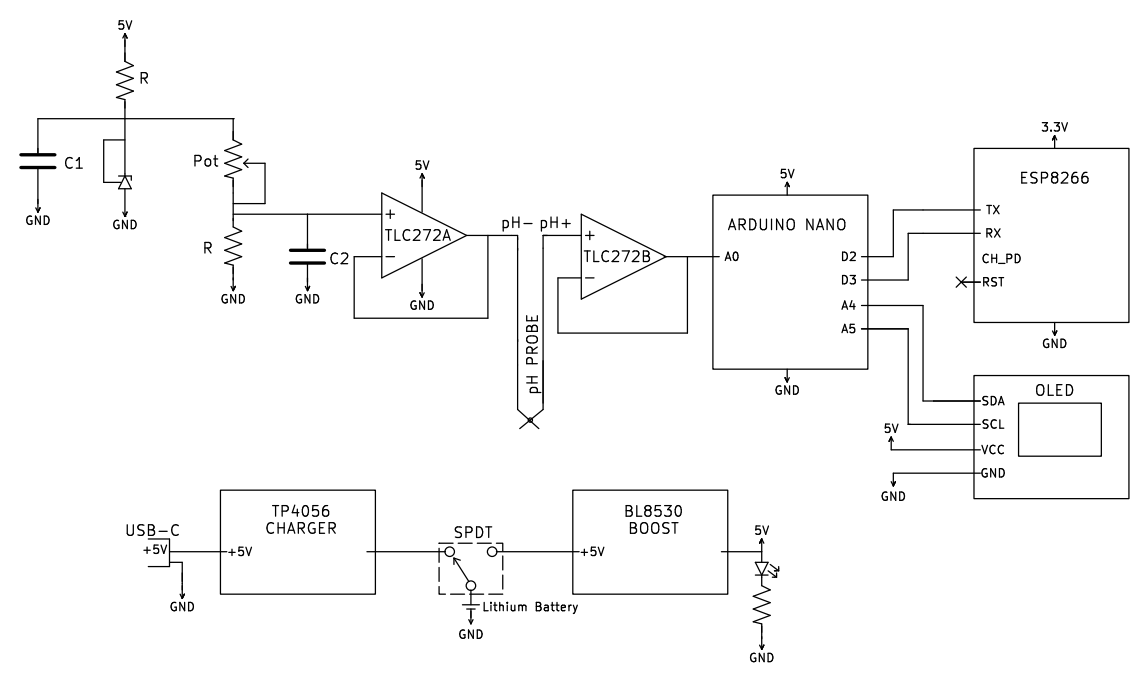
\includegraphics[width=0.7\textwidth]{images/block_diagram.png}}
  \caption{Block diagram of the digital pH meter system}
\end{figure}

% ------------------------------
\section{Schematic Diagram}
\begin{figure}[H]
  \centering
  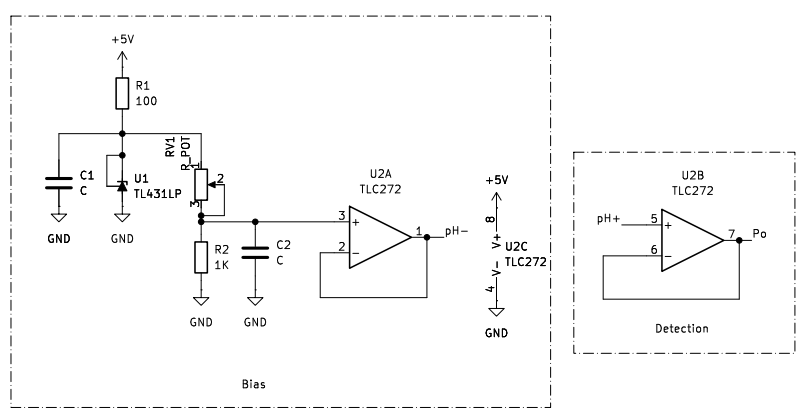
\includegraphics[width=0.9\textwidth]{images/schematic_digram.png}
  \caption{Analog front-end schematic for pH sensing (bias and detection stages)}
\end{figure}

% ------------------------------
\section{Working Principle}
The analog front-end consists of two main sections:
\begin{enumerate}
  \item \textbf{Bias Network:} Establishes a mid-supply reference at \SI{2.5}{\volt} using an accurate voltage reference and resistor divider, shifting the pH probe signal into the ADC range.
  \item \textbf{Amplification Stage:} A differential amplifier built around the TLC4502 scales the \SIrange{-600}{600}{\milli\volt} probe output into a 0--\SI{5}{\volt} span suitable for the Arduino Nano's ADC. A potentiometer allows offset calibration.
\end{enumerate}

The conditioned voltage is then read by the Arduino Nano (using its AREF pin set to the \SI{2.5}{\volt} reference). An ESP8266 module handles wireless transmission of pH data, and an OLED display shows real-time readings.


\newpage
% ------------------------------
\section{Conclusion}
A prototype analog front-end for a digital pH meter was implemented and tested on a breadboard using a \SI{2.5}{\volt} reference and TLC4502 op-amps. The circuit buffers and scales pH probe signals in the \SIrange{-600}{600}{\milli\volt} range into a 0--\SI{5}{\volt} window for the Arduino Nano. Testing with an actual pH probe is pending and will be essential for full system validation. Future integration with the ESP8266 and OLED display will enable wireless, real-time pH monitoring.

 100;1K;
% ------------------------------
\section{Bill of Material}
\begin{table}[H]
\centering
\begin{tabular}{|c|l|c|c|}
\hline
\textbf{S No.} & \textbf{Component} &\textbf{Value}                & \textbf{Quantity} \\ \hline
1 & Arduino Nano & - & 1 \\
2 & TLC4502 Dual Op-Amp & - & 1 \\
3 & Resistor & 1\,k\si{\ohm} & 1\\
4 & Resistor & 100\si{\ohm}& 1\\
5 & Potentiometer & 100\,k\si{\ohm} & 1\\
6 & Capacitor & 0.1uF & 1\\  
6 & Capacitor & 10uF & 1\\   
7 & OLED Display & - & 1    \\
8 & BL8530 &  - & 1 \\          
\hline
\end{tabular}
\caption{Components used in the digital pH meter project}
\end{table}

\end{document}
